%% -------------------------------------------------------
%% Kapitel 5: Backend-Implementierung
%% -------------------------------------------------------
\chapter{Backend-Implementierung}
\label{chap:backend}

\section{Projektstruktur}
\label{sec:projektstruktur}

Das Backend-Projekt (\texttt{Backend.csproj}) ist als ASP.NET~Core~8 Web-API angelegt und
folgt einer klaren Verzeichnisstruktur:

\begin{itemize}
  \item \texttt{Models/} – C\#-Entitätsklassen (\texttt{Dog}, \texttt{Owner}, \texttt{Breed},
    \texttt{LegalRestrictions})
  \item \texttt{Data/} – \texttt{DoggoContext} (DbContext) sowie Seed-Daten als JSON
  \item \texttt{Migrations/} – automatisch generierte EF~Core-Migrationsdateien
  \item \texttt{Utility/} – Hilfsdienste (\texttt{BreedSeeder})
  \item \texttt{Program.cs} – Anwendungseinstiegspunkt und Service-Konfiguration
  \item \texttt{Dockerfile} – Multi-Stage-Build für Docker-Deployment
\end{itemize}

\section{Datenbankmodelle}
\label{sec:modelle}

\subsection{Owner}
\label{subsec:model-owner}

\texttt{Owner} repräsentiert eine registrierte Nutzerin / einen registrierten Nutzer.
Passwörter werden niemals im Klartext gespeichert; stattdessen werden \texttt{PasswordHash}
und \texttt{PasswordSalt} als \texttt{byte[]} persistiert.

\begin{lstlisting}[language=csharp, caption={Modell Owner.cs}, label=lst:owner, float=h]
public class Owner
{
    public Guid Id { get; set; }
    public string Name { get; set; }
    public string Email { get; set; }
    public byte[] PasswordHash { get; set; }
    public byte[] PasswordSalt { get; set; }
    public string? PhoneNumber { get; set; } = null!;

    // Navigation property
    public ICollection<Dog> Dogs { get; set; } = new List<Dog>();
}
\end{lstlisting}

\subsection{Dog}
\label{subsec:model-dog}

\texttt{Dog} hält Name, Alter sowie Fremdschlüssel zu \texttt{Owner} und \texttt{Breed}.
Navigations-Properties ermöglichen EF~Core, die Daten bei Bedarf per \texttt{Include()}
einzulesen.

\begin{lstlisting}[language=csharp, caption={Modell Dog.cs}, label=lst:dog, float=h]
public class Dog
{
    public Guid Id { get; set; }
    public string Name { get; set; }
    public int Age { get; set; }
    public Guid BreedId { get; set; }
    public Guid OwnerId { get; set; }

    public Owner Owner { get; set; } = null!;
    public Breed Breed { get; set; } = null!;
}
\end{lstlisting}

\subsection{Breed und LegalRestrictions}
\label{subsec:model-breed}

\texttt{Breed} verknüpft einen Rassennamen mit einer Beschreibung und einem
\texttt{LegalRestrictions}-Objekt. Letzteres speichert die Vorschriften als
\texttt{List<string>}, die Npgsql auf \texttt{text[]} in PostgreSQL mappt.

\begin{lstlisting}[language=csharp, caption={Modelle Breed.cs und LegalRestrictions.cs}, label=lst:breed, float=h]
public class Breed
{
    public Guid Id { get; set; }
    public string BreedName { get; set; } = null!;
    public string Description { get; set; } = null!;
    public Guid LegalRestrictionsId { get; set; }
    public LegalRestrictions LegalRestrictions { get; set; } = null!;
}

public class LegalRestrictions
{
    public Guid Id { get; set; }
    public string Category { get; set; } = null!;
    public List<string> Rules { get; set; } = new();
}
\end{lstlisting}

\section{DoggoContext und Beziehungskonfiguration}
\label{sec:dbcontext}

Der \texttt{DoggoContext} erbt von \texttt{DbContext} und registriert alle vier
\texttt{DbSet}-Eigenschaften. Die Beziehungen und Constraints werden in
\texttt{OnModelCreating} explizit konfiguriert, um keine unerwünschten Standardverhalten
zu riskieren:

\begin{lstlisting}[language=csharp, caption={DoggoContext.cs – Beziehungskonfiguration (Auszug)}, label=lst:context, float=h]
protected override void OnModelCreating(ModelBuilder modelBuilder)
{
    // Owner -> Dog: 1:N, Cascade Delete
    modelBuilder.Entity<Dog>()
        .HasOne(d => d.Owner)
        .WithMany(o => o.Dogs)
        .HasForeignKey(d => d.OwnerId)
        .OnDelete(DeleteBehavior.Cascade);

    // Dog -> Breed: N:1, Restrict Delete
    modelBuilder.Entity<Dog>()
        .HasOne(d => d.Breed)
        .WithMany()
        .HasForeignKey(d => d.BreedId)
        .OnDelete(DeleteBehavior.Restrict);

    // Unique Index auf Owner.Email
    modelBuilder.Entity<Owner>()
        .HasIndex(o => o.Email)
        .IsUnique();

    // Breed -> LegalRestrictions: N:1, Restrict Delete
    modelBuilder.Entity<Breed>()
        .HasOne(b => b.LegalRestrictions)
        .WithMany()
        .HasForeignKey(b => b.LegalRestrictionsId)
        .OnDelete(DeleteBehavior.Restrict);
}
\end{lstlisting}

\section{EF Core Migrations}
\label{sec:migrations}

Das Datenbankschema wird über EF~Core~Code-First-Migrations verwaltet. Die
Initialmigration \texttt{InitDatabase} erstellt die vier Tabellen \texttt{LegalRestrictions},
\texttt{Owners}, \texttt{Breeds} und \texttt{Dogs} mit allen Constraints und Foreign-Keys.
Neue Schemaänderungen (z.\,B.\ neue Spalten oder Entitäten) werden durch
\texttt{dotnet ef migrations add <Name>} erzeugt und durch \texttt{dotnet ef database update}
auf die laufende Datenbank angewendet. Beim Start der Anwendung wird die Datenbank
automatisch migriert.

\section{Breed-Seeding}
\label{sec:seeding}

Damit beim ersten Start sofort eine vollständige Rassenliste verfügbar ist, liest der
\texttt{BreedSeeder} beim Anwendungsstart \texttt{Data/breeds.json} ein und befüllt die
Tabellen \texttt{LegalRestrictions} und \texttt{Breeds}. Der Seeder prüft zunächst, ob
bereits Einträge vorhanden sind, um eine Mehrfach-Einspielung zu verhindern:

\begin{lstlisting}[language=csharp, caption={BreedSeeder.cs – Idempotentes Seeding}, label=lst:seeder, float=h]
public static async Task SeedBreedsAsync(
    DoggoContext context, string jsonFilePath)
{
    if (context.Breeds.Any()) return; // bereits befuellt

    var jsonData = await File.ReadAllTextAsync(jsonFilePath);
    var breeds = JsonSerializer.Deserialize<List<Breed>>(jsonData,
        new JsonSerializerOptions { PropertyNameCaseInsensitive = true });

    if (breeds != null)
    {
        await context.Breeds.AddRangeAsync(breeds);
        await context.SaveChangesAsync();
    }
}
\end{lstlisting}

Die JSON-Datei enthält pro Rasse einen \texttt{breedName}, eine \texttt{description} sowie
ein \texttt{legal\_restrictions}-Objekt mit \texttt{category} und einem \texttt{rules}-Array.
Listing~\ref{lst:breeds-json} zeigt einen Auszug:

\begin{lstlisting}[language={}, caption={breeds.json – Auszug (Bullterrier)}, label=lst:breeds-json, float=h]
{
  "breedName": "Bullterrier",
  "description": "Muskuloeser Hund mit eifoermigem Kopf.",
  "legal_restrictions": {
    "category": "spezielle_hunderasse",
    "rules": [
      "Mindestalter des Halters: 16 Jahre",
      "Sachkundeausbildung erforderlich",
      "Alltagstauglichkeitspruefung (ATP) verpflichtend",
      "Leinen- und Maulkorbpflicht im oeffentlichen Raum"
    ]
  }
}
\end{lstlisting}

\section{Authentifizierung mit JWT}
\label{sec:auth}

Die Authentifizierung basiert auf \textbf{JSON Web Tokens (JWT)}. Der Ablauf gliedert
sich in zwei Schritte: Registrierung und Anmeldung.

\subsection{Passwort-Hashing}
\label{subsec:passwort-hashing}

Beim Registrieren wird das Passwort mit \textbf{HMAC-SHA512} und einem zufällig generierten
Salt gehasht. Sowohl Hash als auch Salt werden als \texttt{byte[]} in der
\texttt{Owner}-Entität gespeichert. Das Klartext-Passwort verlässt den Request-Scope nie:

\begin{lstlisting}[language=csharp, caption={Passwort-Hashing (Registrierung, Auszug)}, label=lst:hash, float=h]
using var hmac = new HMACSHA512();
owner.PasswordSalt = hmac.Key;
owner.PasswordHash = hmac.ComputeHash(
    Encoding.UTF8.GetBytes(registerDto.Password));
\end{lstlisting}

\subsection{JWT-Ausstellung}
\label{subsec:jwt}

Nach erfolgreicher Anmeldung wird ein JWT mit konfigurierbarer Ablaufzeit und dem
serverseitigen Secret signiert. Das Token enthält den \texttt{NameIdentifier}-Claim mit
der Owner-ID:

\begin{lstlisting}[language=csharp, caption={JWT-Ausstellung (Login, Auszug)}, label=lst:jwt, float=h]
var claims = new[]
{
    new Claim(ClaimTypes.NameIdentifier, owner.Id.ToString()),
    new Claim(ClaimTypes.Email, owner.Email)
};
var key = new SymmetricSecurityKey(
    Encoding.UTF8.GetBytes(configuration["Jwt:Secret"]!));
var token = new JwtSecurityToken(
    issuer: configuration["Jwt:Issuer"],
    audience: configuration["Jwt:Audience"],
    claims: claims,
    expires: DateTime.UtcNow.AddHours(8),
    signingCredentials: new SigningCredentials(
        key, SecurityAlgorithms.HmacSha256));
\end{lstlisting}

\section{Program.cs – Anwendungskonfiguration}
\label{sec:programcs}

\texttt{Program.cs} konfiguriert die Service-Registrierungen und die Middleware-Pipeline:

\begin{lstlisting}[language=csharp, caption={Program.cs (vereinfacht)}, label=lst:program, float=h]
var builder = WebApplication.CreateBuilder(args);

builder.Services.AddDbContext<DoggoContext>(options =>
    options.UseNpgsql(
        builder.Configuration.GetConnectionString("DefaultConnection")));

builder.Services.AddControllers();
builder.Services.AddEndpointsApiExplorer();
builder.Services.AddSwaggerGen();

var app = builder.Build();

// Datenbankmigrationen und Seeding beim Start
using (var scope = app.Services.CreateScope())
{
    var context = scope.ServiceProvider
        .GetRequiredService<DoggoContext>();
    context.Database.Migrate();
    await BreedSeeder.SeedBreedsAsync(context, "Data/breeds.json");
}

app.UseSwagger();
app.UseSwaggerUI();
app.UseHttpsRedirection();
app.UseAuthentication();
app.UseAuthorization();
app.MapControllers();
app.Run();
\end{lstlisting}

\section{Docker-Deployment}
\label{sec:docker}

\subsection{Dockerfile (Multi-Stage-Build)}
\label{subsec:dockerfile}

Das \texttt{Dockerfile} verwendet einen Multi-Stage-Build, um ein möglichst kleines
Produktions-Image zu erzeugen. In der Build-Stage wird das Projekt mit dem .NET~8~SDK
kompiliert; in der finalen Stage wird nur die ASP.NET~Runtime benötigt:

\begin{lstlisting}[language={}, caption={Dockerfile – Multi-Stage-Build (Auszug)}, label=lst:dockerfile, float=h]
FROM mcr.microsoft.com/dotnet/aspnet:8.0 AS base
WORKDIR /app
EXPOSE 8080

FROM mcr.microsoft.com/dotnet/sdk:8.0 AS build
WORKDIR /src
COPY ["Backend/Backend.csproj", "Backend/"]
RUN dotnet restore "Backend/Backend.csproj"
COPY . .
WORKDIR "/src/Backend"
RUN dotnet build "./Backend.csproj" -c Release -o /app/build

FROM build AS publish
RUN dotnet publish "./Backend.csproj" -c Release -o /app/publish

FROM base AS final
WORKDIR /app
COPY --from=publish /app/publish .
ENTRYPOINT ["dotnet", "Backend.dll"]
\end{lstlisting}

\subsection{Docker Compose}
\label{subsec:compose}

\texttt{compose.yaml} startet zwei Services: die PostgreSQL-Datenbank und das Backend.
Das Datenbank-Volume \texttt{postgres\_data} sorgt dafür, dass Daten zwischen Container-Neustarts
erhalten bleiben:

\begin{lstlisting}[language={}, caption={compose.yaml}, label=lst:compose, float=h]
version: '3.8'
services:
  postgres:
    image: postgres:latest
    environment:
      POSTGRES_USER: doggo
      POSTGRES_PASSWORD: doggoGO123
      POSTGRES_DB: doggo_db
    ports:
      - "5432:5432"
    volumes:
      - postgres_data:/var/lib/postgresql/data
  backend:
    build: .
    ports:
      - "8080:8080"
    depends_on:
      - postgres
    environment:
      ConnectionStrings__DefaultConnection: >
        Host=postgres;Port=5432;Database=doggo_db;
        Username=doggo;Password=doggoGO123

volumes:
  postgres_data:
\end{lstlisting}

Mit \texttt{docker compose up --build} werden beide Services gestartet. Das Backend
wartet durch den \texttt{depends\_on}-Eintrag auf die Datenbank, bevor die
Verbindung aufgebaut wird.

\section{Controller-Implementierung}
\label{sec:controller}

Die eigentliche HTTP-Schnittstelle des Backends wird durch ASP.NET~Core~Controller realisiert.
Jeder Controller erbt von \texttt{ControllerBase} und wird mit den Attributen
\texttt{[ApiController]} und \texttt{[Route("api/[controller]")]} annotiert.
\texttt{[ApiController]} aktiviert automatische Modellvalidierung und standardisierte
Fehlerresponses; \texttt{[Route]} legt das URL-Präfix fest (z.\,B.\ \texttt{/api/owners},
\texttt{/api/dogs}).

\subsection{OwnersController}
\label{subsec:owners-controller}

Der \texttt{OwnersController} stellt die Endpunkte für Registrierung und Anmeldung bereit.
Beide Aktionen sind öffentlich zugänglich (kein \texttt{[Authorize]}-Attribut), da eine
Authentifizierung vor der Anmeldung nicht möglich ist:

\begin{lstlisting}[language=csharp, caption={OwnersController – Register und Login (Auszug)}, label=lst:owners-ctrl]
[ApiController]
[Route("api/[controller]")]
public class OwnersController : ControllerBase
{
    private readonly DoggoContext _context;
    private readonly IConfiguration _config;

    public OwnersController(DoggoContext context, IConfiguration config)
    {
        _context = context;
        _config  = config;
    }

    [HttpPost("register")]
    public async Task<IActionResult> Register(RegisterDto dto)
    {
        if (await _context.Owners.AnyAsync(o => o.Email == dto.Email))
            return Conflict("E-Mail-Adresse bereits vergeben.");

        using var hmac = new HMACSHA512();
        var owner = new Owner
        {
            Id           = Guid.NewGuid(),
            Name         = dto.Name,
            Email        = dto.Email,
            PasswordSalt = hmac.Key,
            PasswordHash = hmac.ComputeHash(
                               Encoding.UTF8.GetBytes(dto.Password))
        };
        _context.Owners.Add(owner);
        await _context.SaveChangesAsync();
        return CreatedAtAction(nameof(GetById),
                               new { id = owner.Id }, owner);
    }

    [HttpPost("login")]
    public async Task<IActionResult> Login(LoginDto dto)
    {
        var owner = await _context.Owners
            .FirstOrDefaultAsync(o => o.Email == dto.Email);
        if (owner == null) return Unauthorized();

        using var hmac = new HMACSHA512(owner.PasswordSalt);
        var hash = hmac.ComputeHash(
                       Encoding.UTF8.GetBytes(dto.Password));
        if (!hash.SequenceEqual(owner.PasswordHash))
            return Unauthorized();

        return Ok(new { token = CreateJwt(owner) });
    }
}
\end{lstlisting}

Die Methode \texttt{Register} prüft zunächst per LINQ-Query, ob die E-Mail-Adresse
bereits vergeben ist, und antwortet mit \texttt{409~Conflict}, falls dies der Fall ist.
Bei der Anmeldung (\texttt{Login}) wird das eingegebene Passwort mit dem gespeicherten
HMAC-SHA512-Hash verglichen. Stimmen sie nicht überein, liefert der Endpunkt
\texttt{401~Unauthorized} ohne weitere Details – eine bewusste Designentscheidung, um
keine Hinweise darauf zu geben, ob die E-Mail-Adresse registriert ist.

\subsection{DogsController und Autorisierung}
\label{subsec:dogs-controller}

Alle Endpunkte des \texttt{DogsController} sind mit \texttt{[Authorize]} geschützt. Das
bedeutet, dass der ASP.NET~Core Middleware-Stack das \texttt{Authorization}-Header-Token
vor jedem Aufruf validiert. Ist kein gültiges JWT vorhanden, antwortet die API automatisch
mit \texttt{401~Unauthorized}, bevor die Controllermethode überhaupt ausgeführt wird.

Um sicherzustellen, dass Nutzer\-innen und Nutzer ausschließlich ihre eigenen Hundeprofile
verwalten können, wird die \texttt{OwnerId} nicht aus dem Request-Body gelesen, sondern
direkt aus den JWT-Claims extrahiert:

\begin{lstlisting}[language=csharp, caption={DogsController – OwnerId aus JWT-Claims (Auszug)}, label=lst:dogs-ctrl]
[ApiController]
[Route("api/[controller]")]
[Authorize]
public class DogsController : ControllerBase
{
    private readonly DoggoContext _context;

    public DogsController(DoggoContext context)
        => _context = context;

    private Guid GetCurrentOwnerId() =>
        Guid.Parse(User.FindFirstValue(ClaimTypes.NameIdentifier)!);

    [HttpGet]
    public async Task<IActionResult> GetAll()
    {
        var ownerId = GetCurrentOwnerId();
        var dogs = await _context.Dogs
            .Where(d => d.OwnerId == ownerId)
            .Include(d => d.Breed)
            .ToListAsync();
        return Ok(dogs);
    }

    [HttpDelete("{id}")]
    public async Task<IActionResult> Delete(Guid id)
    {
        var ownerId = GetCurrentOwnerId();
        var dog = await _context.Dogs
            .FirstOrDefaultAsync(d => d.Id == id
                                   && d.OwnerId == ownerId);
        if (dog == null) return NotFound();

        _context.Dogs.Remove(dog);
        await _context.SaveChangesAsync();
        return NoContent();
    }
}
\end{lstlisting}

Die Hilfsmethode \texttt{GetCurrentOwnerId()} liest den \texttt{NameIdentifier}-Claim aus
dem validierten JWT. Da dieser Claim beim Login serverseitig eingetragen wird (Listing
\ref{lst:jwt}), ist er fälschungssicher – der Client kann die \texttt{OwnerId} nicht
manipulieren. Das \texttt{Delete}-Beispiel zeigt außerdem, wie eine
Berechtigungsprüfung auf Datensatzebene erfolgt: Die LINQ-Query filtert gleichzeitig nach
\texttt{Id} und \texttt{OwnerId}, sodass ein fremdes Hundeprofil zuverlässig \texttt{404~NotFound}
zurückgibt, statt eine Fehlermeldung über fehlende Rechte preiszugeben.

\section{API-Dokumentation mit Swagger}
\label{sec:swagger}

Alle Endpunkte werden automatisch durch \textbf{Swashbuckle} (Swagger) dokumentiert und
sind unter \texttt{/swagger} erreichbar. Im Entwicklungsmodus können Endpunkte direkt
aus der Swagger-UI heraus getestet werden. Für gesicherte Endpunkte kann dort ein
Bearer-Token hinterlegt werden. Abbildung~\ref{fig:swagger} zeigt die Swagger-UI mit
den verfügbaren Endpunkten.

\begin{figure}[H]
  \centering
  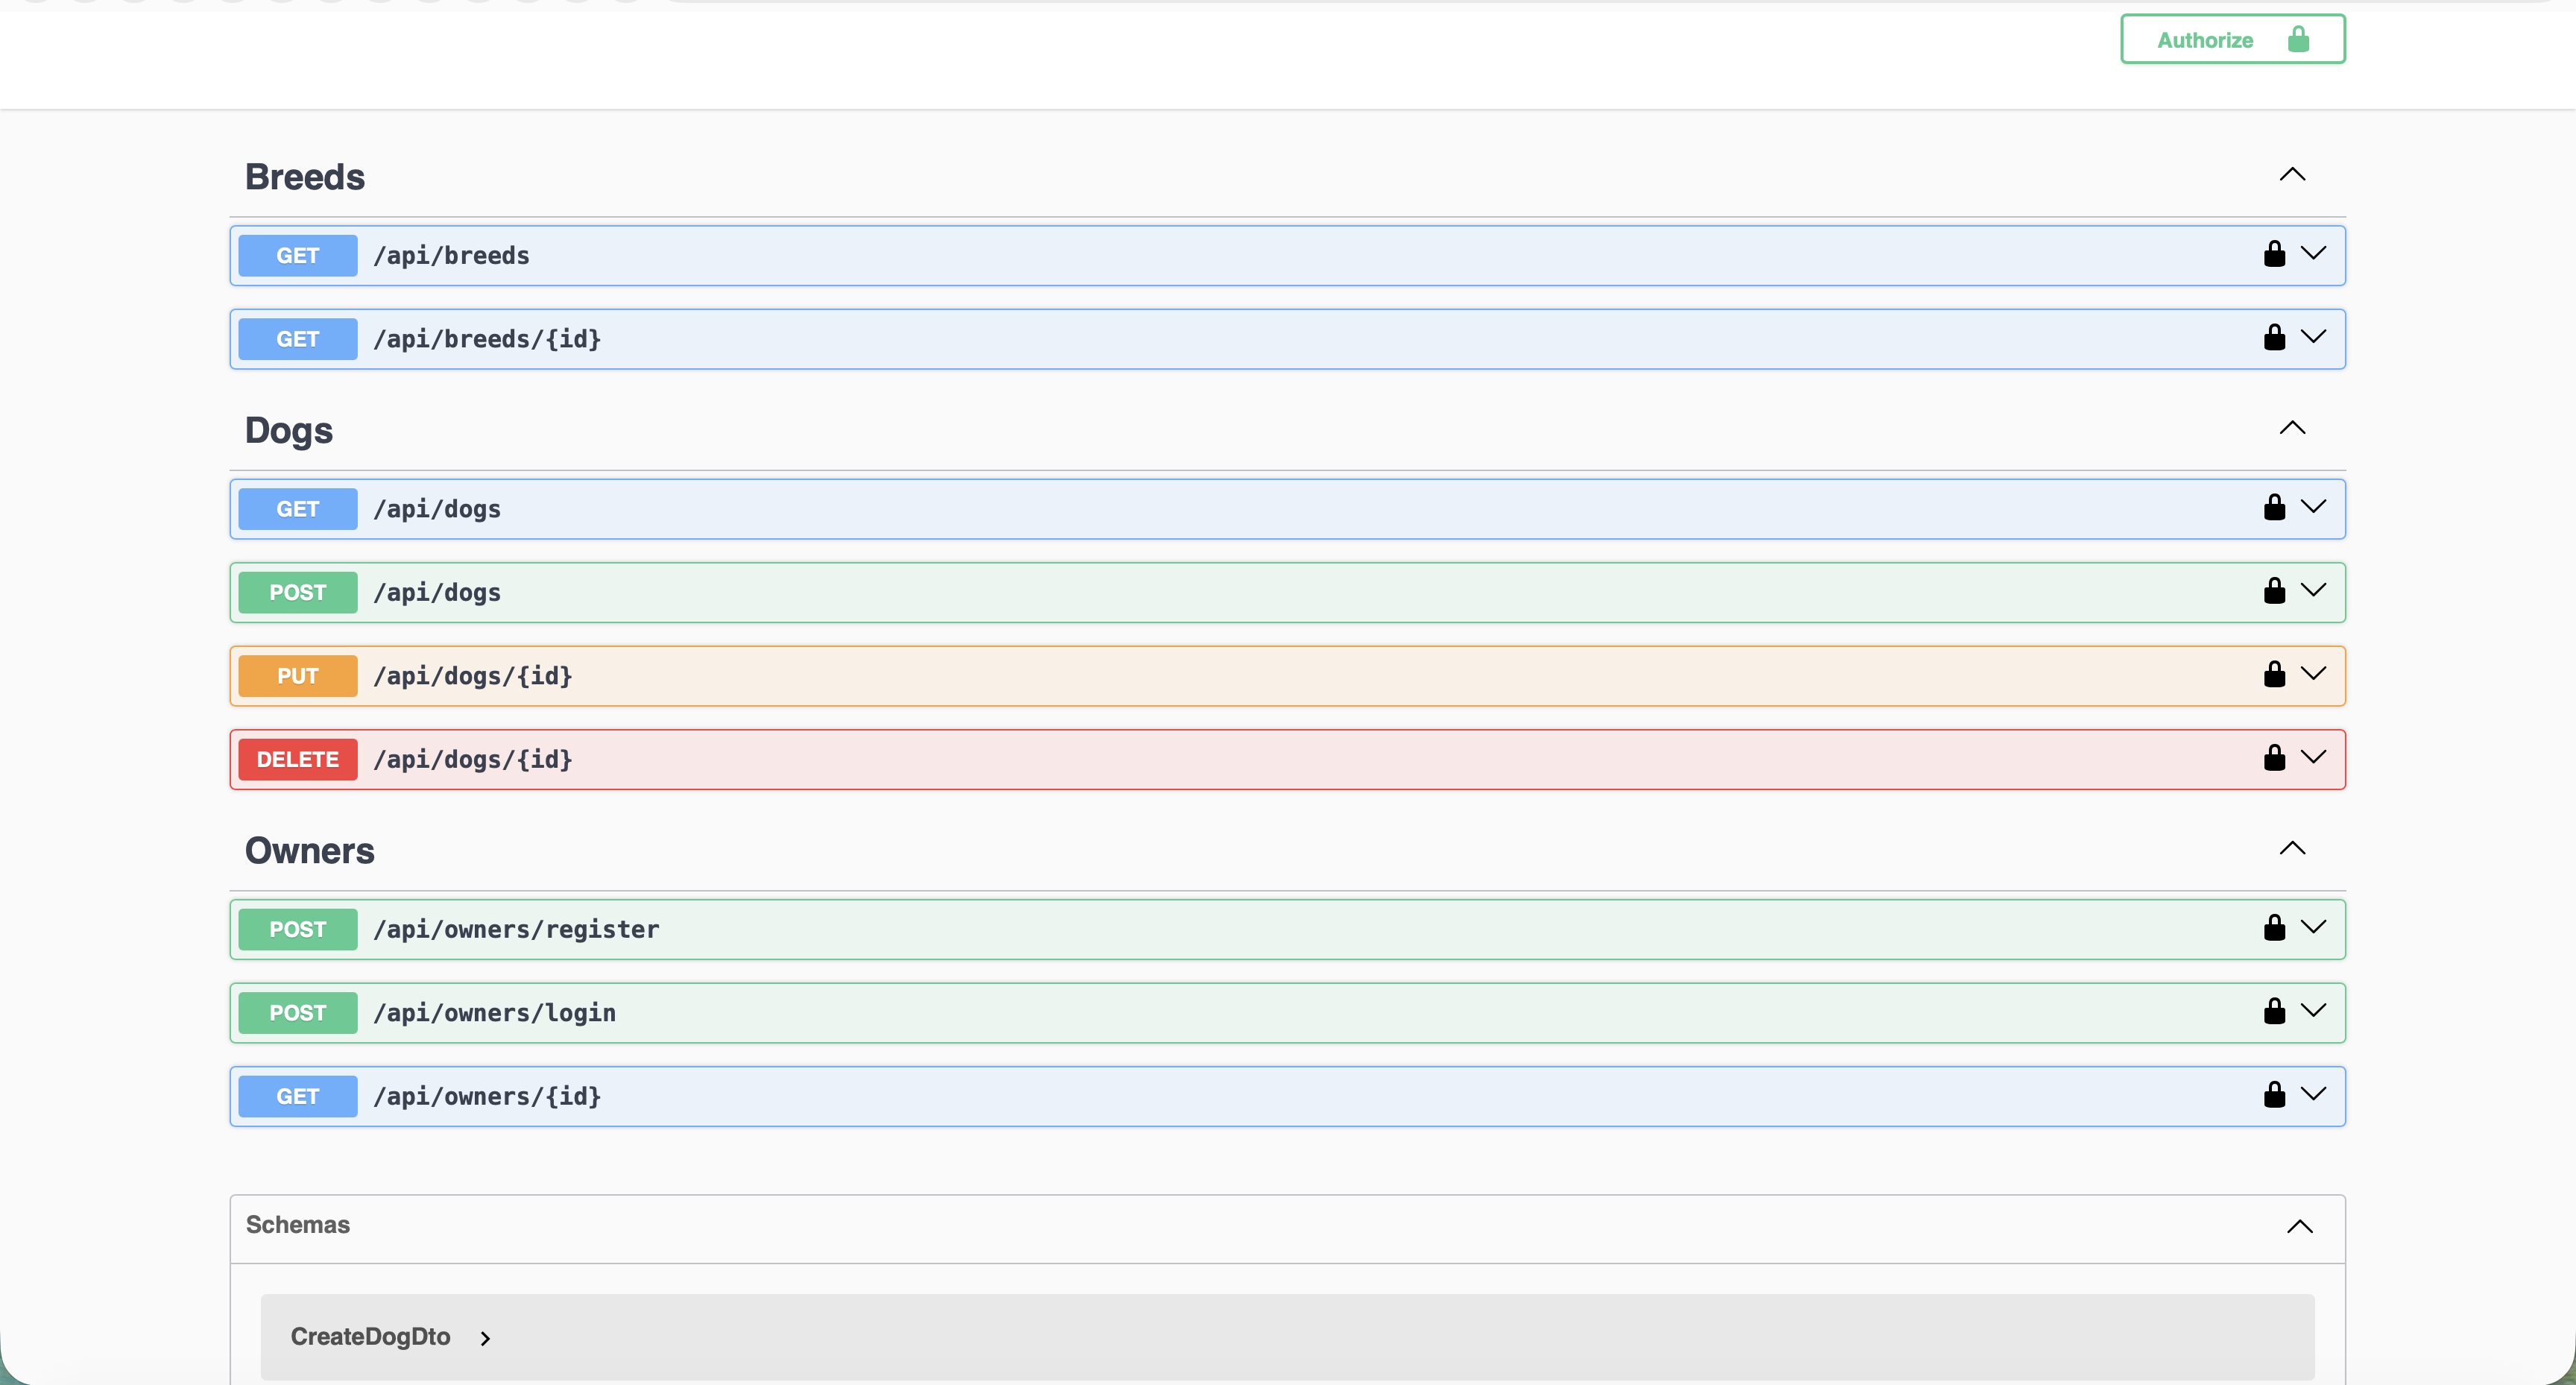
\includegraphics[width=0.9\textwidth]{images/swagger_screenshot.png}
  \caption{Swagger-UI des DoggoGO-Backends}
  \label{fig:swagger}
\end{figure}
